\documentclass[12pt, a4paper]{report}
\usepackage[top=1.5cm, bottom=1.5cm, left=1.5cm, right=1.5cm, columnsep=1cm]{geometry}
% table
\usepackage{booktabs}
\usepackage{multirow}
\usepackage{makecell}
% code
\usepackage{listings} % insert code
\usepackage{xcolor}	 % code color
\definecolor{codegreen}{rgb}{0, 0.6, 0}
\definecolor{codegray}{rgb}{0.5,0.5,0.5}
\definecolor{codepurple}{rgb}{0.58,0,0.82}
\definecolor{backcolour}{rgb}{0.95,0.95,0.92}
\lstset{
backgroundcolor=\color{backcolour}, 
commentstyle=\color{codegreen},
keywordstyle=\color{magnenta},
numbers=left, %行号在左侧显示
numberstyle= \small\color{codegray},%行号字体
numbersep=5pt,
rulesepcolor= \color{gray!80}, %代码块边框颜色
breaklines=true,  %代码过长则换行
keywordstyle= \color{blue},%关键字颜色
frame=shadowbox,	%用方框框住代码块
showspaces=false,
showstringspaces=false,
showtabs=false,
tabsize=1
}

\usepackage{graphicx}
\usepackage{tikz}

\usepackage{fontspec} % require LuaLatex engine
\setmainfont{Times New Roman}

\usepackage{hyperref}
\usepackage{float}
\usepackage{enumitem}

% reference
\usepackage{natbib}
\setcitestyle{authoryear,open={(},close={)}}

\usepackage{amssymb}
%---end preamble---

\begin{document}
\title{\textbf{Comparison between Languages}}
\author{Shark Deng}
\date{March 4 2019}
\maketitle

\begin{abstract}
Development of compilers, such as clang and llvm, booms many computer languages. To name a few, java, swift, php, go, javascript, html, python, c, c++, c\#. In this article, we will go through building blocks of a language. With these elements, we may pick up a new language very quickly or even can create one by llvm.
\end{abstract}

\tableofcontents

\chapter{Computer Language}
\section{Overview}
	Languages can be divided into these categories:
	\begin{description}
		\item[C Familiy] C, C++, C\#, Objective-C
		\item[Based on C] Java, Javascript, Swift, Php, Python
		\item[ML] XML, HTML, YAML
		\item[SQL(Structured Query Language)]  MySql
		\item[Shell] AppleScript
		\item[Other] Latex, Markdown
	\end{description}
	Swift has several features \citep{swift}:
	\begin{enumerate}
	    \item Tuples
	    \item Multiple return values
	    \item Structs that support methods, extensions, and protocols
	    \item Variables are always initialized before use
	\end{enumerate}
	

	
	\subsection{Oriented}
	Object Oriented Programming(OOP)\footnote{https://www.programiz.com/python-programming/object-oriented-programming}, composed of attributes and behaviors, includes four aspects: encapsulation, inheritance, and polymorphism.
	\begin{table}[H]
	\begin{tabular}{l|l}
	\toprule
	Encapsulation & Hiding the private details of a class from other objects. \\
	\hline
	Inheritance & A process of using details from a new class without modifying existing class.\\
	\hline
	Polymorphism & A concept of using common operation in different ways for different data input. \\
	\bottomrule
	\end{tabular}
	\caption{Source: https://www.programiz.com/python-programming/object-oriented-programming}
	\end{table}
	
	\begin{description}
		\item[Object-oriented] C++, C\#, Objective-C, Java, Javascript, Python,Php
		\item[Procedure-oriented] C
		\item[Protocol-oriented] Swift
		\item[Graphic-oriented] Swift
	\end{description}
	
	
		
	\subsection{Compile}
	Phases of compiling are illustrated in Figure \ref{fig:compiling}. LLVM serves as IR. 
	\begin{figure}[H]
	    \centering
	    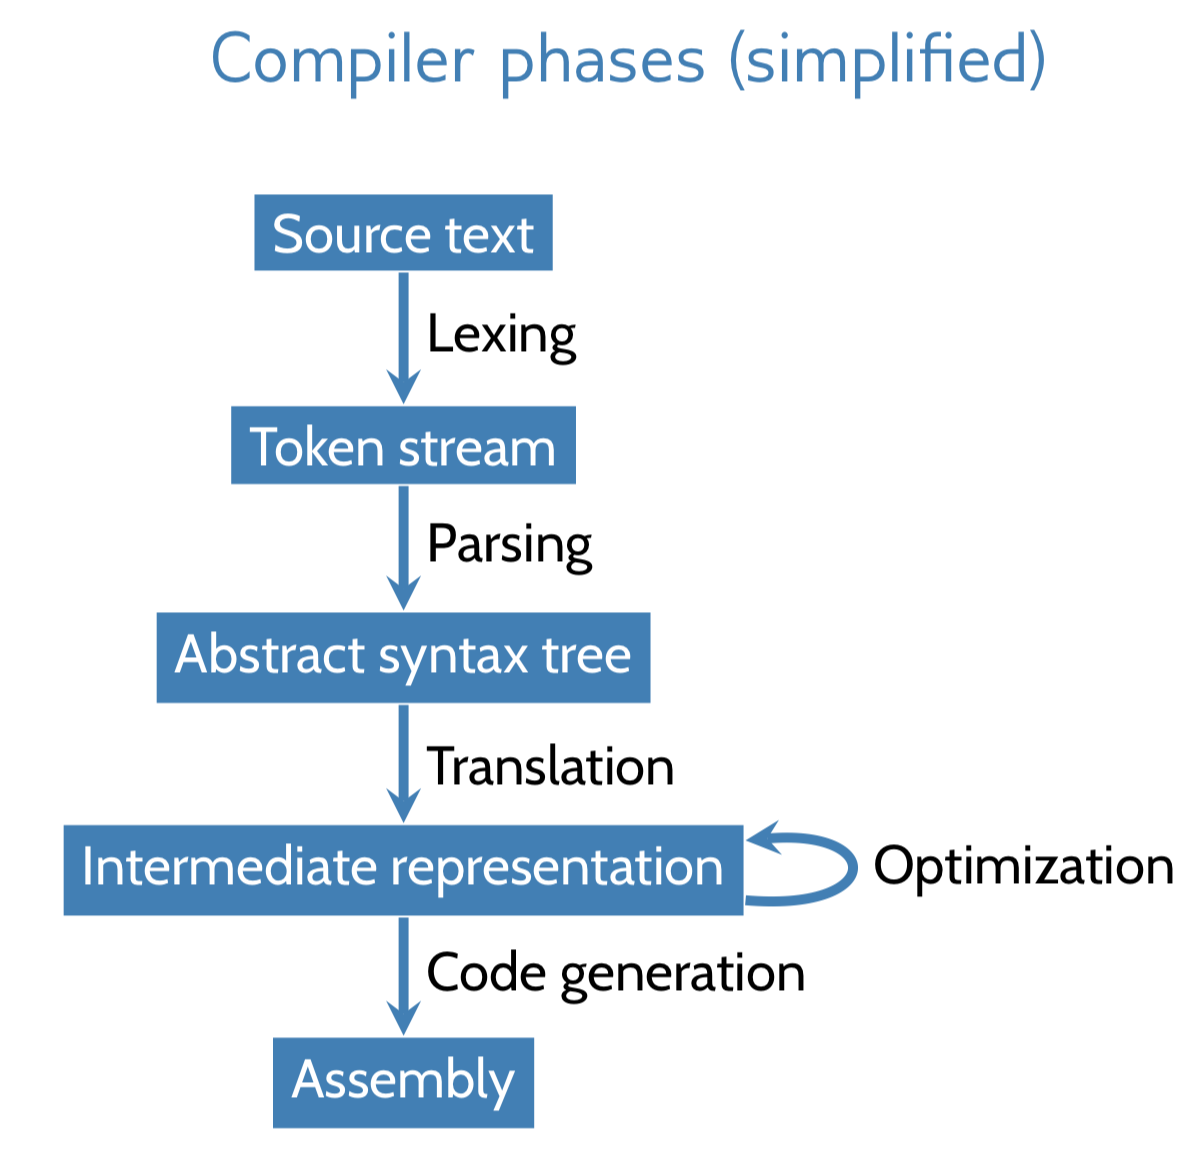
\includegraphics[width=0.3\textwidth]{imgs/phases.png}
	    \caption{\citep{compile}}
	    \label{fig:my_label}
	\end{figure}
	Table \ref{tab:options} will give an overview of three compile forms in these discussed languages.
	\begin{table}[H]
	    \centering
	    \begin{tabular}{c|c|c|c}
	        \toprule
	         Languages & Code on terminal & Compile file on terminal & Code on IDE  \\
	         \hline
	         Java & No & Yes & Yes \\
	         \hline
	         Swift & Yes & Yes & Yes \\
	         \hline
	         Python & Yes & Yes & Yes \\
	         \bottomrule
	    \end{tabular}
	    \caption{Caption}
	    \label{tab:options}
	\end{table}
	
		\subsubsection{Java}
		    \begin{figure}[H]
		        \centering
		        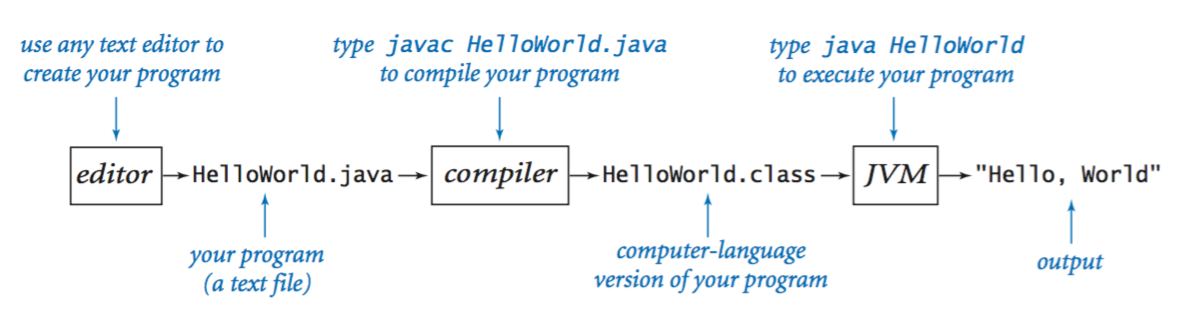
\includegraphics[width=0.8\textwidth]{imgs/developing.png}
		        \caption{\citep{javaCheetsheet}}
		        \label{fig:compiling}
		    \end{figure}
		    \begin{enumerate}
		        \item \textbf{Code on terminal}: \quad None \par 
		        \item \textbf{Compile file on terminal} 
		        \begin{lstlisting}
				$ javac HelloWorld.java
				$ java HelloWorld
			    \end{lstlisting}
			    \item \textbf{Code on IDE}: \quad IntelliJ. Features of the editor will be illustrated in the end.\par 
			    \item \textbf{Product}: \quad .jar 
		    \end{enumerate}
			
		\subsubsection{Swift}
		    \begin{enumerate}
		        \item \textbf{Code on terminal}: \quad Yes \par 
		        \begin{lstlisting}[language=swift]
				$ swift
Welcome to Apple Swift version 4.2.1. Type :help for assistance.
				1> var a = 88
a: Int = 88
				2> let b = 66
b: Int = 66
				3> let c = "Hello!"
c: String = "Hello!"
				4> let d = c + String(b)
d: String = "Hello!66"
				5> import Foundation
		    	\end{lstlisting}
		    	Control + d to exit. 
		    	\item \textbf{Compile file on terminal}: \quad Yes \par 
		    	Swift can be directly as an executable file. Just add the line \colorbox{lightgray}{#!/usr/bin/swift} on top of the file. And use \colorbox{lightgray}{chmod +x fibonacci.swift} to allow the file has executive right. Run \colorbox{lightgray}{./fobonacci.swift} to execute the file. Sample code is from \citep{swiftCompile}.
		    	\item \textbf{Code on IDE}: \quad Xcode \par 
		    	\item \textbf{Product}: \quad .app \par 
		    \end{enumerate}
			 
		
		\subsubsection{Python}
	        \begin{enumerate}
	            \item \textbf{Code on terminal}  \par 
	            Yes
	            \begin{lstlisting}[language=python]
	$ python
	>>> print("Hello World")
	>>> a = 10
	>>> import tensorflow
	>>> quit()
    			\end{lstlisting}
    			\item \textbf{Compile file on terminal} 
    			\begin{lstlisting}
	$ touch a.py
	$ echo "print('Hello World')" >  a.py
    $ cat a.py 	
	$ python a.py
	$ rm a.py
    			\end{lstlisting}
    			\item \textbf{Code on IDE} \par 
    			Pycharm 
	        \end{enumerate}
			
		\subsubsection{Objective-C}
		    \begin{enumerate}
		        \item \textbf{Code on terminal} 
		        \item \textbf{Compile file on terminal}
		        \begin{lstlisting}
    $ touch source.m
	$ gcc -framework Foundation source.m -o source
	$ ./source
    			\end{lstlisting}
		        \item \textbf{Code on IDE} \textbf{Xcode}\par 
		    \end{enumerate}
			
		\subsubsection{Php}
		\begin{enumerate}
		    \item \textbf{Code on IDE}: \quad \textbf{PhpStorm}\par
        \end{enumerate}
		    
        \subsubsection{C}
        \begin{enumerate}
            \item \textbf{Code on IDE}: \quad  \textbf{Xcode}\par 
        \end{enumerate}
		    
        \subsubsection{C++}
        \begin{enumerate}
            \item \textbf{Code on IDE}: \quad \textbf{UE4}\par 
        \end{enumerate}
        
        \subsubsection{C\#}
        \begin{enumerate}
            \item \textbf{Code on IDE}: \quad \textbf{Unity}\par 
        \end{enumerate}
        
			
		
	\subsection{Scalability}
		\subsubsection{Java}
		Some languages have rich libraries. \par
		\begin{lstlisting}
		
		\end{lstlisting}
		\textbf{Dependency Management} \par
		Maven.
		
		\subsubsection{Swift}
		\begin{lstlisting}
		import Foundation
		\end{lstlisting}
		\textbf{Dependency Management} \par
		Codpods
		
		\subsubsection{Python}
		Every file in Python is \textbf{module} \par
		\textbf{Dependency Management} \\
		.yml

	\subsection{Annotation}
	    \subsubsection{Python}
	    It uses \textbf{\#} to annotate single line and \textbf{'''} for multiple lines.

	\subsection{Comments}
	\begin{table}[H]
	    \centering
	    \begin{tabular}{c|c|c}
	        \toprule
	        Language & Single Line & Multiple Line \\
	        \hline
	        HMTL & <!-- -->  & \\
	        \bottomrule
	    \end{tabular}
	    \caption{Caption}
	    \label{tab:my_label}
	\end{table}
	
	

\section{Variable}
    \subsection{Category}
    \textbf{Strong or weak} type means whether the language must specify its variable type. Swift is strong type because it’s designed to run fast.So most of type check works is on programmers and IDE. Php, however, use Zend engine especially universal variable \emph{zval} to parse variables, so its speed will be mush slower. C combines \textbf{strong and weak} types. In normal programming, it needs designate type but in micro programming, type is missed. Other languages, such as Java is strong type.\par 
    Static or dynamic type means whether the variable check is conducted during compile or run time.
    \textbf{Generic} means whether the type can be assigned to various type. \par
    \begin{table}[H]
        \centering
        \begin{tabular}{c|c|c|c}
             \toprule
             Language & Strong or Weak & Static or Dynamic & Support Generic \\
             \hline
             C & Strong & & \\
             \hline
             C(micro) & Weak && \\
             \hline
             Swift & Strong  &&\\
             \hline
             Java & Strong  &&\\
             \hline
             Python & Strong && \\
             \hline
             PHP & Weak && \\
             \bottomrule
        \end{tabular}
        \caption{Variable types in different languages}
        \label{tab:my_label}
    \end{table}
    \subsection{Statement}
    According to \citep{javaCheetsheet}, there are three types of statements: declaration, assignment, and initialization. Declaration means.... Assignment means . Initialization means. \par 
    Table \ref{tab:statements} is an overview of variable statements of these discussed languages. ``-'' means there are no specific supplement. 
    \begin{table}[H]
        \centering
        \begin{tabular}{c|c|c|c}
            \toprule
             Languages & Supplement & Statements\\
             \hline
             Java & - & 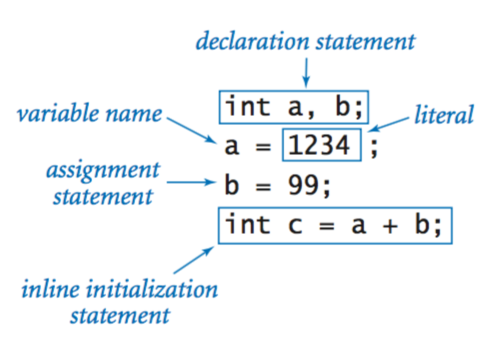
\includegraphics[width=0.3\textwidth]{imgs/assignment.png} \\
             \hline
             \multirow{4}{*}{Swift} & Constant & \colorbox{lightgray}{let a: Int = 1}\\
             & Variable & \colorbox{lightgray}{var a: Int = 1}\\
             & Computed Variable & \\
             & Typealias & \\
             \bottomrule
        \end{tabular}
        \caption{Variable statements}
        \label{tab:statements}
    \end{table}



    
    \subsection{Java}
    \subsubsection{Variable type}
    Java has 4 types of variable. They are:
    \begin{enumerate}
        \item \textbf{Instance}
        \item \textbf{Class} \par 
        Described by \textbf{static} keyword. 
        \item \textbf{Local}
        \item \textbf{Parameter and Argument} \par 
        A formal parameter(also called parameter) is a variable named in the function definition. It will be a local variable that gets initialized as part of the function/method call. \par 
        An actual parameter(also called argument) is a value that is supplied when a function is called. \citep{javaParameter}.
        \begin{lstlisting}
int square(int n) { return n * n; } // n is parameter
System.out.println(square(3)); // 3 is argument
        \end{lstlisting}
        \textbf{Pass argument with value or address} \par 
        Firstly, pass value
        \begin{lstlisting}[language=Java]
public static void main(String[] args) {
    int num1 = 100;
    int num2 = 200;
    take(num1, num2);
    System.out.println("num1 = " + num1);
    System.out.println("num2 = " + num2);
}

public static void take(int a, int b) {
    int temp = a;
    a = b;
    b = temp;
    System.out.println("a = " + a);
    System.out.println("b = " + b);
}
        \end{lstlisting}
        In this case, \emph{a} and \emph{b} \underline{copy} the values of \emph{num1} and \emph{num2}, so changing \emph{a} and \emph{b} doesn't influence \emph{num1} and \emph{num2}.  \par 
        Secondly, pass reference, namely address. 
        \begin{lstlisting}[language=Java]
public static void main(String[] args) {
    int[] intArray = {1,2,3,4,5};
    change(intArray);
    System.out.println(intArray[0]);
}
public static void change(int[] array) {
    int len = array.length;
    array[0] = 0;
}
        \end{lstlisting}
    
        Thirdly, special reference still pass value. 

    \end{enumerate}
    
    \subsubsection{Type Inference}
        \begin{enumerate}
            \item \textbf{Generic}
            \item \textbf{var} keywork \par 
            With the var keyword, Java can infer the type of a local variable from its initialization expression
            \begin{lstlisting}[language=Java]
var theAnswer = 42;
var bike = new Bike();
var mystery; // invalid – no initializer
var nothing = null; // invalid – null has no type
            \end{lstlisting}
            \item \textbf{Lambda}
        \end{enumerate}

    \subsubsection{Data type}
        \begin{enumerate}
            \item \textbf{Primitive data type - 8}
            \begin{table}[H]
        	\centering
	        \begin{tabular}{c|l|l|c|c}
	        \toprule
	        No. & Type & Description & Range & Default \\
	        \toprule
	        1 & byte & 1-byte (8-bit) / signed / 2's complement integer & -128 - 127 & 0 \\
            \hline
	        2 & short & 2-byte (16-bit) / signed / 2's complement & -32768 - 32767 & 0 \\
	        \hline
	        3 & int & 4-byte (32-bit) / signed / 2's complement & $-2^{31} - 2^{31}-1$ & 0 \\
	        \hline
	        4 & long & 8-byte (64-bit) / signed 2's complement & $-2^{63} - 2^{63}-1$ & 0 \\
            \hline
	        5 & float & (32-bit) single precision floating number  & & 0.0f \\
	        \hline
	        6 & double & (64-bit) double precision floating number & & 0.0d \\
	        \hline
	        7 & boolean & logically just a single bit &  true, false & false \\
	        \hline
	        8 & char & 2-byte (16-bit) Unicode character & 0 - 65535  & 0 \\
	        \bottomrule
	        \end{tabular}
	        \caption{Java 8 primitive data types}
	        \end{table}
            \item \textbf{Reference type - 3}
            \begin{table}[H]
                \centering
                \begin{tabular}{c|l|c}
                     \toprule
                     1 & User user & class reference  \\
                     \hline
                     2 & java.lang.Runnable myThread & interface reference \\
                     \hline
                     3 & int[] arr & array reference \\ 
                     \bottomrule
                \end{tabular}
                \caption{3 reference types}
                \label{tab:my_label}
            \end{table}
            
            \item \textbf{Boxing and Unboxing}
            \begin{table}[H]
                \centering
                \begin{tabular}{c|c}
                     &  \\
                     & 
                \end{tabular}
                \caption{Caption}
                \label{tab:my_label}
            \end{table}
        \end{enumerate}
        
        \subsubsection{Modifiers}
        Table below is an overview. 
        \begin{table}[H]
            \centering
            \begin{tabular}{c|c}
                \toprule
                Name & Description \\
                \hline
                public & access control \\
                \hline
                private & access control \\
                \hline
                protected & access control \\
                \hline
                default & access control \\
                \hline
                static & non access \\
                \hline
                final & non access \\
                \hline
                abstract & non access \\
                \hline
                synchronized & thread \\
                \hline
                volatile & thread \\
                \bottomrule
            \end{tabular}
            \caption{Caption}
            \label{tab:my_label}
        \end{table}

    \subsection{Python}
    \_\_name\_\_
    
        \subsubsection{Primitive data type}
        \begin{table}[H]
    	\centering
    	\begin{tabular}{c|l|l|c|c}
    	\toprule
    	No. & Type & Description & Range & Default \\
    	\hline
    	\multirow{4}{*}{1} & \multirow{4}{*}{Number} & int & &  \\
    	& & float & & \\
    	& & bool &  &\\
    	& & complex & & \\
    	\hline
    	2 & String & Non-changeable & & \\
    	\hline
    	3 & Tuple & Non-changeable & & \\
    	\hline
    	4 & List & Changeable & & \\
    	\hline
    	5 & Set & Changeable & & \\	
    	\hline
    	6 & Dictionary & Changeable & & \\
    	\bottomrule
    	\end{tabular}
    	\end{table}
    	Use the code to check type
    	\begin{lstlisting}
    	type(10) # <class 'int'>
    	type(5.5) # <class 'float'>
    	type(True) # <class 'bool'>
    	type(4+3i) # <class 'complex'>
    	isinstance(10, int) # True
    	\end{lstlisting}
    
	
	\subsubsection{C}
	\subsubsection{C++}
	\subsubsection{C\#}
	\subsubsection{Objective-C}
	\footnote{$https://en.wikipedia.org/wiki/C_data_types$}
	
	
\section{Operator}
        \textbf{Arithmetic Operators}
        \begin{table}[H]
            \centering
            \begin{tabular}{c|c|c|c|c}
                \toprule
                No & Operator & Usage & Java & Python \\
                \hline
                1 & + & Addition & \checkmark & \checkmark \\
                \hline
                2 &  - & Minus & \checkmark & \checkmark \\
                \hline
                3 & * &  Multiplication & \checkmark & \checkmark \\
                \hline
                4 & / & Dvision & \checkmark & \checkmark \\
                \hline
                5 & \% & Modulus & \checkmark & \checkmark\\
                \hline
                6 & ++ & & \checkmark & \times \\
                \hline
                7 & $- -$ & Exponent & \checkmark & \times \\
                \hline
                8 & $//$ & Floor division & \times & \checkmark \\
                \bottomrule
            \end{tabular}
            \caption{Arithmetic Operators}
            \label{tab:my_label}
        \end{table}
        
        \textbf{Relational Operators}
            \begin{table}[H]
                \centering
                \begin{tabular}{c|c|c|c|c}
                    \toprule
                    No. & Operator & Usage &Java & Python \\
                    \hline
                    1 & == & Equal to & \checkmark & \checkmark \\
                    \hline
                    2 & != & Not equal to & \checkmark & \checkmark   \\
                    \hline
                    3 & > & Greater than & \checkmark & \checkmark  \\
                    \hline
                    4 & < & Less than & \checkmark & \checkmark  \\
                    \hline
                    5 & >= & Greater than or Equal to  & \checkmark & \checkmark \\
                    \hline
                    6 & <= & Less than or Equal to & \checkmark & \checkmark \\
                    \bottomrule
                \end{tabular}
                \caption{Relational Operators}
                \label{tab:my_label}
            \end{table}
 
        \textbf{Bitwise Operators}
            \begin{table}[H]
                \centering
                \begin{tabular}{c|c|c}
                    \toprule
                    No. & Operator & Usage \\
                    \hline
                    1 & \& &  \\
                    \hline
                    2 & | &  \\
                    \hline
                    3 & \^ & \\
                    \hline
                    4 & \~ & \\
                    \hline
                    5 & << & \\
                    \hline
                    6 & >> & \\
                    \hline
                    7 & >>> & \\
                    \bottomrule
                \end{tabular}
                \caption{Bitwise Operators}
                \label{tab:my_label}
            \end{table}
            
        \subsection{Logical Operators}
            \begin{table}[H]
                \centering
                \begin{tabular}{c|c|c|c|c}
                     \toprule
                    No. & Operator & Usage & Java & Python\\
                    \hline
                    1 & \&\& & and & \checkmark & and  \\
                    \hline
                    2 & || & or & \checkmark & or \\
                    \hline
                    3 & ! & not & \checkmark & not \\
                    \bottomrule
                \end{tabular}
                \caption{Logical Operators}
                \label{tab:my_label}
            \end{table}
            
        \subsection{Assignment Operators}
        \subsection{Misc Operators}
        
        
        
	
\section{Control Flow - 5}	
	\subsection{Selection - 3}
		\subsubsection{If then else}
		\subsubsection{Switch}
		\subsubsection{Try ... except ...}
	\subsection{Iteration - 2}
		\subsubsection{For}
		\subsubsection{While}


\section{Method}
	\subsection{Define}
		\subsubsection{Python}
		\begin{lstlisting}[language={python}]
		def main():
   			print('hello')
			
		main()
		\end{lstlisting}

\section{Class}
	\subsection{Access Level}
		\subsubsection{Swift - 5}
		\begin{table}[H]
		\centering
		\begin{tabular}{|c|c|l|c|}
		\toprule
		name & specifier & access & example \\
		\hline
		open & & outside module (read and modify) & \\
		\hline
		public & & outside module (read) & \\
		\hline
		internal & & inside module & \\
		\hline
		fileprivate & & inside file & \\
		\hline
		private & & inside class & \\
		\bottomrule
		\end{tabular}
		\end{table}
	
		
		\subsubsection{Python - 3}
		\begin{table}[H]
		\centering
		\begin{tabular}{|c|c|l|c|}
		\toprule
		name & specifier & access & example \\
		\hline
		public & - & - & self.public = 10  \\
		\hline
		protected & single underline & - & self.\_protected = 10 \\
		\hline
		private & double underlines & inside this class & self.\_\_private = 10\\
		\bottomrule
		\end{tabular}
		\end{table}
		

	\subsection{Define}
		A class has \textbf{constructor}, \textbf{destructor}. These will be detailed in following table of responding languages:
		\subsubsection{Python}
		Example code for Magic Methods is available here \href{https://github.com/muerbingsha/compsumm/blob/master/learn/python/Test5.py}{Test5.py}
		\begin{table}[H]
		\centering
		\begin{tabular}{|c|l|}
		\toprule
		Magic Methods & Meaning \\
		\toprule
		\_\_new\_\_ & create a new instance \\
		\_\_init\_\_ & constructor(initialize a new instance)  \\
		\_\_del\_\_ & desctructor \\
		\hline
		\_\_str\_\_ & print(obj) \\
		\_\_repr\_\_ & obj(on terminal) \\
		\hline
		\_\_getitem\_\_ & \\
		\_\_setitem\_\_ & \\
		\hline
		\_\_cmp\_\_ & \\
		\_\_eq\_\_ & = \\
		\_\_ne\_\_ & != \\
		\_\_lt\_\_ & < \\
		\_\_gt\_\_ & > \\
		\_\_le\_\_ & <= \\
		\_\_ge\_\_ & >= \\
		\hline
		\_\_add\_\_ & + \\
		\_\_sub\_\_ & - \\
		\_\_floordiv\_\_ & // \\
		\_\_truediv\_\_ & / \\
		\_\_mod\_\_ & \% \\
		\_\_pow\_\_ & ** \\
		\_\_lshift\_\_ & << \\
		\_\_rshift\_\_ & >> \\
		\_\_and\_\_  & \& \\
		\_\_xor\_\_ & \\
		\_\_or\_\_ & \\
		\bottomrule
		\end{tabular}
		\caption{Magic methods}
		\end{table}
		
		Python use \textbf{decorator} to realize static class and so on. Pre-made decorators are listed in the following table \ref{tab-decorator} and relevant example is \href{https://github.com/muerbingsha/compsumm/blob/master/learn/python/Test1.py}{Test1.py}. Custom decorator is exampled here \href{https://github.com/muerbingsha/compsumm/blob/master/learn/python/Test6.py}{Test6.py}. 
		\begin{table}[H]
		\centering
		\begin{tabular}{|l|l|c|}
		\toprule
		Method Decorator & Meaning & Example \\
		\toprule
		@staticmethod &  & \\
		\hline
		@classmethod & &  \\
		\hline
		@property & getter and setter & \href{https://github.com/muerbingsha/compsumm/blob/master/learn/python/Test3.py}{Test3.py} \\
		\bottomrule
		\end{tabular}
		\caption{Pre-made decorators}
		\label{tab-decorator}
		\end{table}
		
		
	\subsection{Java}
	    \textbf{Object} is composed of state and behavior \citep{object}.  \par 
	    An \textbf{interface} is a group of methods without implementations \citep{javaIntro}. Any class that implements MovableThing must include definitions of these methods. \par 
	    \textbf{Inheritance} forms a hierarchy by subclass \textbf{extends} super class\par 
	    A \textbf{package} is a namespace that organizes a set of related classes and interfaces. \par  
	    
	    \subsubsection{Abstract}
	    According to \citep{abstractClass}, an abstract class is a class that is declared abstract, it may or may not include abstract methods. Abstract classes cannot be instantiated, but they can be subclassed. \par 
	    An abstract method is a method that is declared without an implementation (without braces, and followed by a semicolon). \par 
	    Abstract methods can be implemented or declared abstract in subclasses. 
	    \subsubsection{Inheritance}
	    \colorbox{lightgray}{super.parentMethod();}
	    \subsubsection{Interface}
	    \subsubsection{Nested}
	    \subsubsection{Singleton}
	    \subsubsection{Enum}
	    An enum is a special "class" that represents a group of constants (unchangeable variables, like final variables) \citep{javaEnum}. \par 
	    An enum can, just like a class, have attributes and methods. The only difference is that enum constants are public, static and final (unchangeable - cannot be overridden)
	    \lstinputlisting[language=Java]{code/Sample.java}
	    \subsubsection{Annotation}
	    Classes, methods, variables, parameters and Java packages may be annotated.
	    Built-in annotations:
	    @override
	
\section{Exception}


\section{Standard Library}
    \subsection{Java}
        \subsubsection{Comparable \& Comparator}
        \lstinputlisting[language=Java]{code/Movie.java}
     
     \subsection{Python}
     	\subsubsection{Numpy}
		\begin{enumerate}
			\item np.random.shuffle()
			\item np.random.choice()
		
		\end{enumerate}
	
        



\chapter{Data structure and Algorithm}
    Data structure can be divided into linear and non-linear. Linear structure includes array and linked list. Non-linear structure includes tree and graph. \par 
    Data structure has a wide range of applications. For example, when studying natural language processing, Mr. Deng presented that put all study materials, such as thesis, models, code, data sets, and so on in download folder.  \par 
    Abstract data types(ADT) is abstract, not concrete. List, set, map are ADTs. 
    \section{Overview}
        \subsection{Complexity}
        \begin{enumerate}
            \item time
            \item space 
            \item energy
        \end{enumerate}
        Types of complexity: 
        \begin{enumerate}
            \item 
        \end{enumerate}
        How to compute
        \begin{enumerate}
            \item Worst case
            \item Average case
            \item Best case 
        \end{enumerate}
    
        \subsection{Types}
        \begin{enumerate}
            \item Static and Dynamic 
            \begin{enumerate}
                \item Static data structure: size is fixed, such as array.
                \item Dynamic data structure: size is not fixed, such as linked list.
            \end{enumerate}
            \item Linear and non-linear
            \begin{enumerate}
                \item Linear
                \item Non-linear
            \end{enumerate}
        \end{enumerate}
        
        \subsection{Operations}
        \begin{enumerate}
            \item add
            \item remove
            \item get specific node
            \item get size
            \item get whether is empty
            \item get whether is full(only suitable for static type)
            \item foreach all nodes
        \end{enumerate}
    
    \section{List}
    The list ADT is a container known mathematically as a \emph{finite} sequence of elements. List has these 2 characteristics:
    \begin{enumerate}
        \item duplicates are allowed
        \item order is preserved
    \end{enumerate}
    List can be implemented by array, and linked list. Comparisons between them are as follows:
    \begin{enumerate}
        \item array: 
        \begin{enumerate}
            \item easy to look up: O(1)
            \item messy to grow and contract
        \end{enumerate}
        \item linked list:
        \begin{enumerate}
            \item traverse list to find arbitrary element: O(n)
            \item easy to grow, contract
        \end{enumerate}
    \end{enumerate}
    Operations are:
    \lstinputlisting[language=Java]{code/List.java}
        \subsection{Array}
        \subsection{Single linked list}
        \subsection{Double linked list}
        \subsection{Circular single linked list}
        \subsection{Circular double linked list}
    
    \section{Stack}
    
    \section{Queue}
    
    \section{Tree}
    Characteristics: 
    \begin{enumerate}
        \item tree is a node
        \item a node contains \underline{value} and a list of \underline{nodes}
        \item for value, it can be \underline{(key, value)} pair or \underline{single key}.
        \item not allow duplicate items
        \item ordered 
    \end{enumerate}
        \subsection{Binary tree}
        Binary tree is different from binary search tree. Binary tree is each node has at most 2 sub nodes. Binary search tree is binary tree, in which the nodes are sorted, namely the value of the left child node is smaller than the value of the node and the value of the right node is bigger than the value of the node.  \par 
        Complexity: 
        \begin{enumerate}
            \item add
            \item find
            \item remove
            \item foreach
        \end{enumerate}
        \subsection{Binary Search Tree - BST}
        \subsection{Balanced Binary Search Tree - AVL}
        \subsection{Huffman Tree}
        \subsection{Quadtree}
        \subsection{Octree}
        \subsection{Red-Black tree}
        
    
    \section{Graph}
    
    \section{Set}
   	 \begin{enumerate}
       	 	\item not duplicate elements
        		\item unordered collection
    	\end{enumerate}
    
    \section{Map}
    Characteristics:
    \begin{enumerate}
        \item (key, value) pairs
    \end{enumerate}
        \subsection{Java}
        \begin{lstlisting}[language=Java, caption=Map.java]
public interface Map<K, V> {
    V put(K key, V value);
    V get(K key);
    boolean remove(K key);
    void clear();
    int size();
}
        \end{lstlisting}
    \section{Hash Table}
    
    \section{Finding}
    
    \section{Sort}
        \subsection{Merge sort}
        \subsection{Selection sort}
    
    \section{Python}
        \subsection{List}
        \begin{lstlisting}[language=Python]
empty = [] 	# create an empty list
letters = [`a', `b']	# create a list
numbers = [1, 2, 3]
mixed = [`a', 1] 		# list can have mixed members
        \end{lstlisting}
        
        \subsection{Dict}
        \begin{lstlisting}[language=Python]
a = {`Name': `Zhang', `Age': 18, `Menu':[`Fruit', `Vega']}	# create dict
a[`Name']			# visit value
a[`Name'] = `Li'		# modify value
a[`Schools'] = `Jobyme'	# add value
del a['Name']		# delete value
a.clear()			# clear the dict
del a				# delete the dict memory space
        \end{lstlisting}
        
        
        \subsection{Set}
        
        \subsection{Tuple}
        
        \subsection{Collections-namedtuple}
        \begin{lstlisting}[language=Python]
websites = [('Sohu', 'http://www.sohu.com', 'Zhang'), 
		('Sina', 'http://www.sina.com', 'Li'), 
		('Yahoo', 'http://yahoo.com', 'Wu')]
web = namedtuple('Website', ['name', 'url', 'author'])
for w in websites:
	w = web._make(w)
	print(w)
        \end{lstlisting}
        
        \subsection{Collections-dequeue}
        
        \subsection{Collections-Counter}
        
        \subsection{Collections-defaultdict}
        
        \subsection{Collections-OrderedDict}
        

    
\section{Java}
    \subsection{HashSet}
    Characteristics:
    \begin{enumerate}
        \item unordered collection
        \item ignore duplicate items
    \end{enumerate}
    \begin{table}[H]
        \centering
        \begin{tabular}{c|c|l}
            \toprule
            No & Function & API \\
            \hline
            1 & create & HashSet() \\
            & & HashSet(Collection<? extends E> c) \\
            \hline
            2 & add & add(E e) \\
            \hline
            3 & remove & remove(Object o) \\
            & & removeAll(Collection<?> c) \\
            & & removeIf(); \\
            & & clear() \\
            \hline
            4 & get & size() \\
            & & contains(Object o) \\
            & & isEmpty() \\
            \hline
            5 & foreach & \\
            \bottomrule
        \end{tabular}
        \caption{Caption}
        \label{tab:my_label}
    \end{table}
    
    
		
		\href{http://www.jobyme88.com}{stMap.java}


\chapter{Algorithm}
Three aspects to evaluate an algorithm: time, space, and energy. \par 
We consider worst case, best case, and average case for computation complexity. \par 
\begin{table}[H]
    \centering
    \begin{tabular}{c|c}
        \toprule
         Time & Example  \\
         \hline
         Constant O(1) &  \\
         \hline
         Logarithmic O(log(n))& finding an element in a balanced BST \\
         Linear O(n) linked list &  \\
         O(n log(n)) & average time to sort merge sort \\
         \bottomrule
    \end{tabular}
    \caption{Caption}
    \label{tab:my_label}
\end{table}
\section{Greedy Algorithm}
\subsubsection{Fractional Knapsack Problem}
\begin{figure}[H]
    \centering
    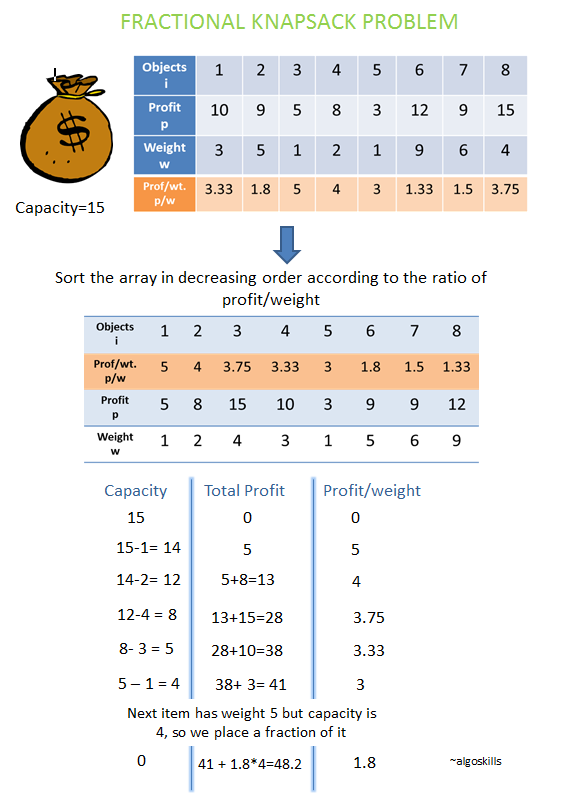
\includegraphics[width=0.5\textwidth]{imgs/backpack.png}
    \caption{Caption}
    \label{fig:my_label}
\end{figure}


\chapter{Core Computer Science}
\section{Basic IO}
\section{Basic data manipulation}
\section{File}
\section{Thread}
In concurrent programming, thread, process, and coroutine are important. \par 
Each process has its own memory space. \par 
Threads share the process's resources, including memory and open files. \par 
Reasons for using threads are concurrency and parallelism. 
    \subsection{Java}
    A Java application can create additional processes using a \textbf{ProcessBuilder} object. \par
    The \textbf{Thread} class is used to create threads and interact with them. \par
    Two ways to create a thread: \citep{thread} 
    \begin{enumerate}
        \item Subclass \underline{Thread},extending its run()method
        \begin{itemize}
            \item Advantages: class inherits all of Thread’s methods
            \item Disadvantages: can’t subclass anything else
        \end{itemize}
        \item Use the \underline{Runnable} interface and implement its run() method.
        \begin{itemize}
            \item General, but does not inherit Thread’s methods
        \end{itemize}
    \end{enumerate}
    Related methods:
    \begin{enumerate}
        \item t.start() will start execution of the run() method within the
thread t. If the there are multiple threads, they will start at the same time.
        \item t.join() will cause the current thread to wait until thread t
terminates. Usually it is the main thread to wait other threads to complete. 
    \end{enumerate}
    Race condition and \underline{synchronized} keyword
    \begin{enumerate}
        \item synchronized is to qualify a method, ensures only one thread executes that method at any time
    \end{enumerate}
    Samples:
    \url{Worker.java}
    \url{Tuna.java}
    

\section{Recursion}
    \subsection{Fibonnaci}

\section{Math}




\section{UI}
    \subsection{Java-JavaFX}
    \subsection{HTML}
    \begin{enumerate}
        % meta
        \item \textbf{<meta>}
        \begin{lstlisting}[language=HTML]
<meta charset="UTF-8">
<meta name="description" content="">
<meta name="keywords" content="">
<meta name="author" content="">
<!-- responsive -->
<meta name="viewport" content="width=device-width, initial-scale=1.0">
<!-- Refresh document every 30 seconds -->
<meta http-equiv="refresh" content="30">
        \end{lstlisting}
        
        \large{\textcolor{blue}{\textbf{Media}}}
        \item \textbf{<audio>(<source>)}
        \underline{controls} shows sound bar
        \begin{lstlisting}[language=HTML]
<audio controls>
    <source src="horse.ogg" type="audio/ogg">
    <source src="horse.mp3" type="audio/mpeg">
</audio>
        \end{lstlisting}
        
\includegraphics[width=0.5\textwidth]{imgs/html_audio.png}
        
        \item \textbf{<video>}
        \begin{lstlisting}[language=HTML]
<video width="400" controls>
    <source src="mov_bbb.mp4" type="video/mp4">
    <source src="mov_bbb.ogg" type="video/ogg">
    Your browser does not support HTML5 video.
</video>
        \end{lstlisting}
        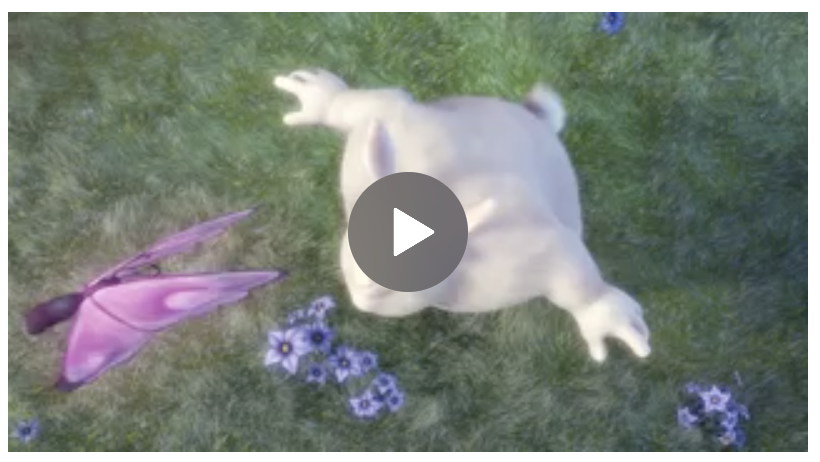
\includegraphics[width=0.5\textwidth]{imgs/html_video.png}
        
        \item \textbf{<iframe>}
        To embed Youtube video, simply right click to get code.
        \begin{lstlisting}[language=HTML]
<iframe width="806" height="453" src="https://www.youtube.com/embed/V1ejrlYY1Qs?list=LL7CoUzO3ZFpw-UbKQhDRweA" frameborder="0" allow="accelerometer; autoplay; encrypted-media; gyroscope; picture-in-picture" allowfullscreen>
</iframe>
        \end{lstlisting}
        
        \item \textbf{<object>}
        It is used to embed plug-ins (like Java applets, PDF readers, Flash Players) in web pages. \citep{html5}
        \begin{lstlisting}[language=HTML]
<object width="400" height="50" data="bookmark.swf"></object>
<object width="100%" height="500px" data="snippet.html"></object>
        \end{lstlisting}
        
        
        \item \textbf{<p>}
        \begin{table}[H]
            \centering
            \begin{tabular}{c|c}
                \toprule
                Tag & Description \\
                \hline
                <i> &  \\
                \hline
                <strong> &  \\
                \hline
                <em> & \\
                \hline
                <u> & underline text \\
                \hline
                <br> & break line \\
                \hline 
                <hr> & horizon line \\
                \hline
                <sub> & subscript text \\
                \hline 
                <sup> & superscript text \\
                <h1> - <h6> & headers \\
                \bottomrule
            \end{tabular}
            \caption{Caption}
            \label{tab:my_label}
        \end{table}
        
        \item \textbf{<pre>}
        \begin{lstlisting}[language=HTML]
<pre>
    My Bonnie lies over the ocean.
    My Bonnie lies over the sea.
    My Bonnie lies over the ocean.
        
    Oh, bring back my Bonnie to me.
</pre>
        \end{lstlisting}
        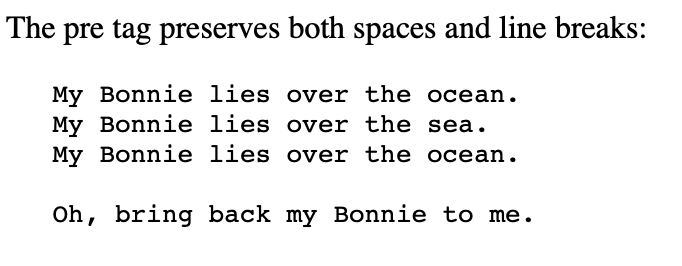
\includegraphics[width=0.3\textwidth]{imgs/html_pre.png}
        
        
        % ul
        \item \textbf{<ul>}: unordered list
        \begin{lstlisting}[language=HTML]
<ul>
    <li>Menu one</li>
    <li>Menu two</li>
</ul>
        \end{lstlisting}
        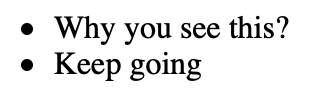
\includegraphics[width=0.2\textwidth]{imgs/html_ul.png}
        % ol
        \item \textbf{<ol>}
        % dl 
        \item \textbf{<dl>}
    
        %% graphic 
        \Large{\textcolor{blue}{\textbf{Graphic}}}
        % svg
        \item \textbf{<svg>}
        
        % canvas
        \item \textbf{<canvas>}
        
        \item \textbf{<a>}
        
        \item \textbf{<img>}
        
        %% html5 semantic
        \Large{\textcolor{blue}{\textbf{HTML 5 Semantic}}}
        \item \textbf{<header>(<article>, <main>, <footer>, <section>, <aside>)}
        \begin{lstlisting}[language=HTML]
<header>
    <nav>
        Nav part
    </nav>
</header>
<main>
    <article>
        <section>
            <aside>
                Section one
            </aside>
        </section>
    </article>
</main>
<footer>
        Copyright &copy 2019
</footer>
        \end{lstlisting}
        
        
        % table
        \item \textbf{<table> (<tr>, <th>, <td>, <thead>, <tbody>, <tfoot>)} \par 
        <tr> defines a row and there are two tabel cells: <th> header cell and <td> standard cell. \par 
        The <thead>, <tbody>, and <tfoot> will not affect the layout of the table by default. However, you can use CSS to style these elements.
        \begin{lstlisting}[language=HTML, caption=table.html]
<!DOCTYPE html>
<html>
    <head>
    <style>
    thead {color:green;}
    tbody {color:blue;}
    tfoot {color:red;}
    table, th, td {
      border: 1px solid black;
    }
    </style>
    </head>
    <body>
    <table>
      <thead>
        <tr>
          <th>Month</th>
          <th>Savings</th>
        </tr>
      </thead>
      <tbody>
        <tr>
          <td>January</td>
          <td>$100</td>
        </tr>
        <tr>
          <td>February</td>
          <td>$80</td>
        </tr>
      </tbody>
      <tfoot>
        <tr>
          <td>Sum</td>
          <td>$180</td>
        </tr>
      </tfoot>
    </table>
    </body>
</html>
        \end{lstlisting}
        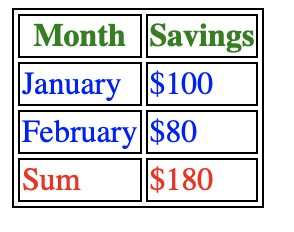
\includegraphics[width=0.3\textwidth]{imgs/html_table.png}
        
        % form
        \item \textbf{<form>}
        \begin{lstlisting}[language=HTML]
<form action="/action_page.php">
    First name: <input type="text" name="FirstName" value="Mickey"><br>
    Last name: <input type="text" name="LastName" value="Mouse"><br>
    <input type="submit" value="Submit">
</form>
        \end{lstlisting}
        
        % select
        \item \textbf{<select>(<optgroup>, <option>} \par 
        A drop-down list 
        \begin{lstlisting}[language=HTML]
<select>
    <optgroup label="Swedish Cars">
        <option value="volvo">Volvo</option>
        <option value="saab">Saab</option>
    </optgroup>
    <optgroup label="German Cars">
        <option value="mercedes">Mercedes</option>
        <option value="audi">Audi</option>
    </optgroup>
</select>
        \end{lstlisting}
        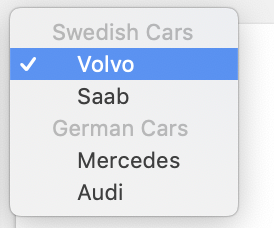
\includegraphics[width=0.3\textwidth]{imgs/html_select.png}
        
        % detail
        \item \textbf{<detail>(<summary>)}
        \begin{lstlisting}[language=HTML]
<details>
    <summary>Copyright 1999-2014.</summary>
    <p> - by Refsnes Data. All Rights Reserved.</p>
    <p>All content and graphics on this web site are the property of the company Refsnes Data.</p>
</details>
        \end{lstlisting}
        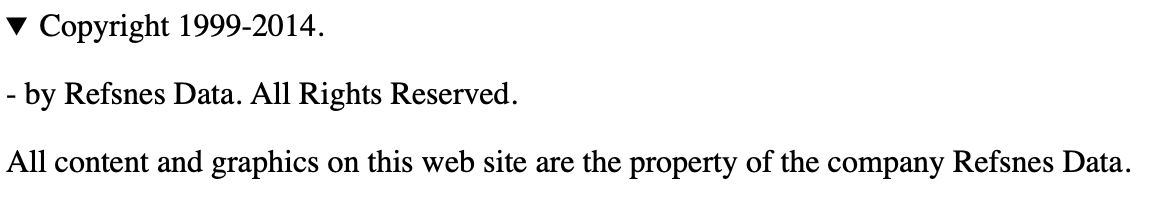
\includegraphics[width=0.6\textwidth]{imgs/html_detail.png}
        
        \item \textbf{<dialog>}
        
        \item \textbf{<menu>}
        
        
        
    \end{enumerate}





\chapter{Software Industry}
\section{IDE}
    \subsection{Java-IntelliJ}
    \subsection{Swift-Xcode}
    \subsection{C\#-Unity}
    \subsection{C++-UE4}
    \subsection{Python-Pycharm}
\section{Version Control}
    \begin{enumerate}
        \item Commit
        \item Push
        \item Pull
        \item Update
        \item Revert
    \end{enumerate}
    
\section{Test}
    \subsection{Java-Junit}
    \subsection{Swift-UITest}
    \subsection{Python-pytest}
    
\section{Debug}

\section{Code Naming Tradition}
    \subsection{Java}
    \begin{enumerate}
        \item case-sensitive
        \item Whitespace not permitted
        \item special characters are forbidden
        \item Java keywords and reserved words cannot be used
        \item Class names start with capital letters
        \item Variable names start with lower case, and use upper case for subsequent words
        \item Constant names use all caps and underscores
    \end{enumerate}
    
\section{Packaging}
\section{Problem Shooting}


\clearpage
\lstlistoflistings

% biblio
% harvard family: dcu / agsm / kluwer
\bibliographystyle{dcu}
\bibliography{ref}

\end{document}